% ╔══════════════════════════════════════════════════════════════════╗
% ║  PROPOSTA TÉCNICO-COMERCIAL — ALERTA FUTUROS                       ║
% ║  App de alertas de trading para Windows (Binance Futuros USDⓈ-M)   ║
% ║  Emitida por: Blumenau TI                                         ║
% ║  Compilar: pdflatex -interaction=nonstopmode proposta-alerta-futuros.tex (2x)
% ╚══════════════════════════════════════════════════════════════════╝
\documentclass[11pt,a4paper]{article}

% ── Encoding & Language ─────────────────────────────────────────────
\usepackage[utf8]{inputenc}
\usepackage[T1]{fontenc}
\usepackage[brazilian]{babel}
\usepackage{textcomp}

% ── Typography ──────────────────────────────────────────────────────
\usepackage{lmodern}
\usepackage[scaled=0.92]{helvet}
\renewcommand{\familydefault}{\sfdefault}
\usepackage[tracking=true,kerning=true]{microtype}

% ── Page Layout ─────────────────────────────────────────────────────
\usepackage[a4paper, top=28mm, bottom=30mm, left=24mm, right=24mm, headheight=20mm]{geometry}
\usepackage{fancyhdr}
\usepackage{lastpage}
\usepackage{parskip}
\setlength{\parskip}{7pt}

% ── Cores (paleta Blumenau TI) ──────────────────────────────────────
\usepackage{xcolor}
\definecolor{navy}    {HTML}{0B1426}
\definecolor{navymid} {HTML}{1E3A5F}
\definecolor{gold}    {HTML}{FFB700}
\definecolor{golddk}  {HTML}{B7791F}
\definecolor{cyan}    {HTML}{00B4D8}
\definecolor{cyandk}  {HTML}{0E7490}
\definecolor{txtgray} {HTML}{4A5568}
\definecolor{lightbg} {HTML}{F1F5F9}
\definecolor{borderc} {HTML}{CBD5E1}
\definecolor{sinalW}  {HTML}{16A34A}
\definecolor{sinalZ}  {HTML}{DC2626}
\definecolor{amber}   {HTML}{A05F00}

% ── Symbols ─────────────────────────────────────────────────────────
\usepackage{pifont}
\usepackage{marvosym}
\usepackage{amssymb}
\newcommand{\icoCheck} {\textcolor{sinalW}{\ding{51}}}
\newcommand{\icoCross} {\textcolor{sinalZ}{\ding{55}}}
\newcommand{\icoBullet}{\textcolor{cyandk}{\ding{108}}}
\newcommand{\icoStar}  {\textcolor{gold}{\ding{72}}}
\newcommand{\icoBolt}  {\textcolor{golddk}{\Lightning}}
\newcommand{\icoV}     {\textcolor{cyandk}{\textbf{V1}}}
\newcommand{\usdm}{USD\raisebox{0.15ex}{\textcircled{\raisebox{-0.05ex}{\tiny S}}}-M}

% ── Resultados medidos na PoC (execução ao vivo) ────────────────────
\newcommand{\pocData}{16/09/2026, 19h25--20h25}
\newcommand{\pocMin}{60}
\newcommand{\pocAval}{88}
\newcommand{\pocSinais}{16}
\newcommand{\pocLatMed}{637}
\newcommand{\pocLatPnf}{3.184}
\newcommand{\pocLatMax}{3.268}
\newcommand{\pocReconex}{1}
\newcommand{\pocRam}{39}

% ── Cliente e autoria ───────────────────────────────────────────────
\newcommand{\cliente}{Roberto Urbano}
\newcommand{\autor}{Eng. Lucas William Junges}
\newcommand{\autorLinkedinURL}{https://www.linkedin.com/in/lucas-william-junges-a95b00143/}
\newcommand{\autorLinkedin}{linkedin.com/in/lucas-william-junges-a95b00143}

% ── Valores comerciais ──────────────────────────────────────────────
\newcommand{\valPoc}{390,00}
\newcommand{\valA}{999,00}
\newcommand{\valB}{1.799,00}
% saldo após abater a PoC e parcelas 50/50 (manter coerente com os totais acima)
\newcommand{\valAsaldo}{609,00}
\newcommand{\valBsaldo}{1.409,00}
\newcommand{\valAparc}{304,50}
\newcommand{\valBparc}{704,50}
\newcommand{\valSuporte}{89,00}
\newcommand{\valHora}{120,00}

% ── Graphics & Tables ───────────────────────────────────────────────
\usepackage{graphicx}
\usepackage{tikz}
\usetikzlibrary{arrows.meta,positioning,calc,fit,backgrounds}
\usepackage{booktabs}
\usepackage{tabularx}
\usepackage{array}
\usepackage{colortbl}
\usepackage{fvextra}

% ── Boxes & Decoration ──────────────────────────────────────────────
\usepackage{tcolorbox}
\tcbuselibrary{skins,breakable,raster}
\usepackage{enumitem}
\usepackage{ragged2e}

% ── Links ───────────────────────────────────────────────────────────
\usepackage[hidelinks,
  pdfauthor={Eng. Lucas William Junges (Blumenau TI)},
  pdftitle={Proposta Técnico-Comercial --- Alerta Futuros (App de alertas Binance para Windows)},
  pdfsubject={Aplicativo de alertas de trading com dados públicos da Binance Futuros},
]{hyperref}

% ── Section styles ──────────────────────────────────────────────────
\usepackage{titlesec}
\titleformat{\section}
  {\color{navy}\Large\bfseries}
  {\color{golddk}\thesection.}{10pt}{}[{\color{borderc}\titlerule[0.5pt]}]
\titleformat{\subsection}
  {\color{navymid}\large\bfseries}
  {\color{golddk}\thesubsection.}{8pt}{}
\titlespacing{\section}{0pt}{16pt}{9pt}
\titlespacing{\subsection}{0pt}{12pt}{5pt}

% ── Header / Footer ─────────────────────────────────────────────────
\pagestyle{fancy}
\fancyhf{}
\renewcommand{\headrulewidth}{0pt}
\fancyhead[C]{%
  \begin{tikzpicture}[remember picture, overlay]
    \fill[navy] ([yshift=-14mm]current page.north west) rectangle (current page.north east);
    \fill[gold] ([yshift=-14mm]current page.north west) rectangle ([yshift=-14.8mm]current page.north east);
    \node[anchor=west, text=white, font=\small\bfseries]
      at ([xshift=14mm, yshift=-7mm]current page.north west) {Blumenau\,\textcolor{gold}{TI}};
    \node[anchor=east, text=white!72, font=\small]
      at ([xshift=-14mm, yshift=-7mm]current page.north east) {Proposta Técnico-Comercial --- Alerta Futuros};
  \end{tikzpicture}%
}
\fancyfoot[C]{%
  \begin{tikzpicture}[remember picture, overlay]
    \fill[lightbg] (current page.south west) rectangle ([yshift=8mm]current page.south east);
    \draw[borderc] ([yshift=8mm]current page.south west) -- ([yshift=8mm]current page.south east);
    \node[anchor=west, text=txtgray, font=\scriptsize]
      at ([xshift=14mm, yshift=4mm]current page.south west) {PCT-AF-2026-001 \textbullet\ Confidencial --- uso exclusivo de \cliente};
    \node[anchor=east, text=txtgray, font=\scriptsize]
      at ([xshift=-14mm, yshift=4mm]current page.south east) {Página \thepage\ de \pageref{LastPage}};
  \end{tikzpicture}%
}

% ─── Box styles ─────────────────────────────────────────────────────
\tcbset{
  execbox/.style={enhanced, colback=navy!4, colframe=navymid, arc=6pt, boxsep=7pt, left=6pt, right=6pt,
    fonttitle=\bfseries\color{white}, attach boxed title to top left={yshift=-2mm, xshift=8mm},
    boxed title style={colback=navy, arc=3pt, boxsep=3pt}},
  goldbox/.style={enhanced, breakable, colback=gold!9, colframe=golddk,
    leftrule=4pt, toprule=0.4pt, bottomrule=0.4pt, rightrule=0.4pt, arc=4pt, boxsep=5pt, before upper=\RaggedRight},
  cyanbox/.style={enhanced, colback=cyan!7, colframe=cyandk,
    leftrule=4pt, toprule=0.4pt, bottomrule=0.4pt, rightrule=0.4pt, arc=4pt, boxsep=5pt, before upper=\RaggedRight},
  greenbox/.style={enhanced, colback=sinalW!7, colframe=sinalW,
    leftrule=4pt, toprule=0.4pt, bottomrule=0.4pt, rightrule=0.4pt, arc=4pt, boxsep=5pt, before upper=\RaggedRight},
  ajuste/.style={enhanced, breakable, colback=white, colframe=borderc, arc=4pt, boxsep=4pt,
    leftrule=3pt, colbacktitle=lightbg, coltitle=navy, fonttitle=\bfseries,
    borderline west={3pt}{0pt}{golddk}},
  opcao/.style={enhanced, colback=white, colframe=navymid, arc=6pt, boxsep=5pt,
    fonttitle=\bfseries\color{white}, colbacktitle=navymid, halign title=center},
  opcaorec/.style={enhanced, colback=gold!6, colframe=golddk, arc=6pt, boxsep=5pt,
    fonttitle=\bfseries\color{navy}, colbacktitle=gold, halign title=center},
  pricebox/.style={enhanced, colback=navy, colframe=gold, arc=8pt, boxsep=7pt, left=8pt, right=8pt,
    fontupper=\color{white}},
  terminal/.style={enhanced, colback=navy, colframe=navymid, arc=4pt, boxsep=3pt, left=5pt, right=5pt,
    fontupper=\color{white!90}\ttfamily\fontsize{6.3}{8.1}\selectfont}
}

% ══════════════════════════════════════════════════════════════════════
\begin{document}
\hypersetup{pageanchor=false}
\thispagestyle{empty}

% ╔══════════════════════════════════════════════════════════════════╗
%  CAPA
% ╚══════════════════════════════════════════════════════════════════╝
\begin{tikzpicture}[remember picture, overlay]
  \fill[navy] (current page.south west) rectangle (current page.north east);
  \fill[gold] (current page.north west) rectangle ([yshift=-7mm]current page.north east);
  \fill[gold] (current page.south west) rectangle ([yshift=5mm]current page.south east);
  % "gráfico de velas" decorativo
  \begin{scope}[shift={([xshift=-128mm, yshift=-150mm]current page.north east)}, opacity=0.22]
    \foreach \x/\o/\c/\h/\l [count=\i] in
      {0/20/34/38/16, 9/34/28/40/24, 18/28/46/50/26, 27/46/40/52/36, 36/40/58/62/38,
       45/58/52/64/48, 54/52/70/76/50, 63/70/64/74/58, 72/64/84/90/62, 81/84/78/92/74,
       90/78/96/102/76, 99/96/88/100/84, 108/88/110/118/86}{
      \pgfmathsetmacro{\lo}{min(\o,\c)} \pgfmathsetmacro{\hi}{max(\o,\c)}
      \ifdim \c pt > \o pt \def\cor{sinalW}\else\def\cor{sinalZ}\fi
      \draw[\cor, line width=0.8pt] (\x mm+2.5mm, \l mm) -- (\x mm+2.5mm, \h mm);
      \fill[\cor] (\x mm, \lo mm) rectangle (\x mm+5mm, \hi mm);
    }
  \end{scope}
  \fill[cyan!12] ([xshift=-20mm, yshift=60mm]current page.south west) circle (40mm);
\end{tikzpicture}

\vspace*{16mm}
\begin{center}
  {\color{gold}\scriptsize\bfseries\MakeUppercase{Proposta Técnico-Comercial}}\\[3mm]
  {\color{white!80}\scriptsize N.\textsuperscript{o} PCT-AF-2026-001 \quad\textbullet\quad 16 de setembro de 2026}

  \vspace{58mm}

  {\color{white}\fontsize{36}{42}\bfseries\selectfont Alerta Futuros}\\[4mm]
  {\color{gold}\fontsize{15}{20}\bfseries\selectfont App de alertas de trading para Windows}\\[3mm]
  {\color{white!75}\normalsize Dados públicos da Binance Futuros \usdm\ em tempo real\\
   sem conta, sem API key, sem senha e sem envio de ordens}

  \vspace{10mm}
  \begin{tikzpicture}
    \draw[gold, line width=1.5pt] (0,0) -- (3.5cm,0);
    \fill[gold] (1.75cm,0) circle (2.5pt);
    \draw[gold!40, line width=0.5pt] (3.5cm,0) -- (7.5cm,0);
  \end{tikzpicture}
  \vspace{10mm}

  \begin{tikzpicture}
    \node[fill=white, fill opacity=0.07, text opacity=1, draw=gold, line width=1pt,
          rounded corners=8pt, inner sep=12pt] {%
      \color{white}
      \begin{minipage}{82mm}\centering
        {\bfseries\large Blumenau\,\textcolor{gold}{TI}}\\[4pt]
        {\small\color{white!75} www.blumenauti.com.br}\\[2pt]
        {\small\color{white!75} contato@blumenauti.com.br \;\textbullet\; +55 47 98867-7798}\\[6pt]
        {\color{gold!60}\rule{50mm}{0.4pt}}\\[5pt]
        {\footnotesize\color{white!85} Documento elaborado pelo \textbf{\color{white}\autor}}\\[2pt]
        {\scriptsize\href{\autorLinkedinURL}{\color{gold}\autorLinkedin}}
      \end{minipage}};
  \end{tikzpicture}

  \vspace{12mm}
  {\color{white!55}\footnotesize
    Preparada para \textbf{\color{white!90}\cliente} --- projeto \textbf{\color{white!85}APP-Futuros}\\[2mm]
    Inclui \textbf{\color{gold}Prova de Conceito (PoC) já em funcionamento}
    \textbullet\ Válida por \textbf{\color{gold}30 dias}}
\end{center}

\newpage
\hypersetup{pageanchor=true}
\setcounter{page}{1}

% ══════════════════════════════════════════════════════════════════════
%  SUMÁRIO EXECUTIVO
% ══════════════════════════════════════════════════════════════════════
\vspace*{2mm}
\begin{tcolorbox}[execbox, title={Sumário Executivo}]
  Você descreveu, com bastante precisão, um aplicativo que fica ``de vigia'' no mercado de
  Futuros da Binance e avisa na tela quando dois critérios se cruzam: o \textbf{RSI de 2
  períodos na vela de 5 minutos} e a \textbf{posição do preço dentro da vela de 15 minutos}.
  Quando a condição é verdadeira, aparece um pop-up com o par e o \textbf{Preço-Alvo}
  (verde ou vermelho), por 10 segundos.

  \vspace{3pt}
  Antes de enviar esta proposta, \textbf{construímos e testamos uma Prova de Conceito (PoC)}
  com a sua regra, conectada à Binance real:

  \begin{itemize}[leftmargin=1.6em, itemsep=3pt, topsep=2pt]
    \item[\icoCheck] Os \textbf{8 pares} (BTC, ETH, SOL, BNB, XRP, LINK, LTC e DOGE) monitorados ao
      mesmo tempo, por \textbf{uma única conexão} e \textbf{só com dados públicos}.
    \item[\icoCheck] \textbf{\pocAval\ fechamentos de 5 minutos} avaliados em \pocMin\ minutos ao vivo,
      \textbf{\pocSinais\ sinais reais} identificados; uma queda de conexão foi detectada e recuperada sozinha em 4 s.
    \item[\icoCheck] Alerta na tela em \textbf{\pocLatMed\ ms} (mediana) após o fechamento da vela
      --- o cálculo em si leva menos de 1 ms; o restante é o tempo da própria Binance e da internet.
    \item[\icoCheck] Leve: cerca de \textbf{\pocRam\ MB de memória} e menos de 1\% de CPU.
  \end{itemize}

  \vspace{3pt}
  Propomos entregar o app em \textbf{duas etapas}: primeiro a \textbf{PoC instalada no seu
  laptop} (R\$ \valPoc, valor \textbf{100\% abatido} na etapa seguinte), para você conferir os
  números com o gráfico da Binance; depois a \textbf{Versão 1}, em duas opções ---
  \textbf{Essencial} por R\$ \valA\ ou \textbf{Completa} por R\$ \valB\ ---, com entrega em
  \textbf{5 a 8 dias úteis}.
\end{tcolorbox}

\vspace{4mm}
\begin{tcbraster}[raster columns=4, raster equal height, raster column skip=3mm]
  \newcommand{\kpi}[2]{\begin{tcolorbox}[enhanced, colback=navy, colframe=navy, arc=5pt, boxsep=3pt, halign=center, valign=center]
    {\color{gold}\LARGE\bfseries #1}\\[1mm]{\color{white!80}\scriptsize #2}\end{tcolorbox}}
  \kpi{8}{pares ao mesmo tempo}
  \kpi{0,6\,s}{até o alerta (mediana)}
  \kpi{\pocRam\,MB}{de memória}
  \kpi{5--8}{dias úteis de entrega}
\end{tcbraster}

\newpage
% ══════════════════════════════════════════════════════════════════════
\section{Entendimento do Pedido}
% ══════════════════════════════════════════════════════════════════════

Lemos o documento \emph{APP-Futuros} item por item. A tabela abaixo mostra cada requisito,
como ele é atendido e o que \textbf{já está funcionando na PoC}.

\begin{center}
\small
\renewcommand{\arraystretch}{1.32}
\begin{tabularx}{\textwidth}{@{}>{\raggedright\arraybackslash}p{50mm} >{\raggedright\arraybackslash}X c@{}}
  \toprule
  \rowcolor{navy!8}
  \textbf{Requisito do documento} & \textbf{Como atendemos} & \textbf{PoC} \\
  \midrule
  Somente dados públicos; sem API key, senha ou ordens & Endpoints públicos REST e WebSocket; nenhuma credencial & \icoCheck \\
  Somente Futuros \usdm, pares USDT & Servidores \texttt{fapi}/\texttt{fstream} (Spot ignorado); 8 pares USDT & \icoCheck \\
  Carga histórica via REST ao abrir & Velas de 5m baixadas uma vez por par (ver ajuste 4.1) & \icoCheck \\
  WebSocket contínuo e reconexão automática & Stream combinado, reconexão progressiva e recuperação de velas perdidas & \icoCheck \\
  Avaliar só no fechamento da vela 5m (\texttt{x:\,true}) & Evento oficial de vela encerrada da Binance & \icoCheck \\
  Condição 1 --- RSI(2): Acima 90--100 / Abaixo 0--5 & RSI de Wilder, o mesmo método dos gráficos & \icoCheck \\
  Condição 2 --- Setores A / B / C da vela 15m & 30\% / 40\% / 30\%; vela válida se tamanho $>$ 0,020\% & \icoCheck \\
  Cruzamento X / Y e Preço-Alvo W / Z ($\pm$0,5\%) & Exatamente como descrito & \icoCheck \\
  Pop-up 10 s, verde (W) / vermelho (Z), casas decimais por par & Pop-up próprio no canto inferior direito (ver ajuste 4.4) & \icoCheck \\
  Janela com campos e botões Iniciar / Parar & Opção Completa (Seção 5) & \icoV \\
  Programa instalável no laptop Windows & Executável único \texttt{.exe} para Windows 10 e 11 & \icoV \\
  \bottomrule
\end{tabularx}
\end{center}

% ══════════════════════════════════════════════════════════════════════
\section{Como Funciona --- em Linguagem Simples}
% ══════════════════════════════════════════════════════════════════════

\begin{center}
\begin{tikzpicture}[
  font=\small,
  caixa/.style={draw=navymid, fill=white, rounded corners=4pt, align=center, inner sep=5pt, line width=0.7pt},
  titulo/.style={font=\footnotesize\bfseries, text=navymid},
  seta/.style={-{Stealth[length=2.6mm]}, line width=1pt, color=golddk}]
  % Binance
  \node[caixa, text width=33mm] (rest) {\textbf{Dados de Mercado}\\{\scriptsize REST --- 1 vez, ao abrir}\\{\scriptsize histórico de velas 5m}};
  \node[caixa, text width=33mm, below=6mm of rest] (ws) {\textbf{WebSocket}\\{\scriptsize contínuo, 24 h}\\{\scriptsize velas 5m e 15m ao vivo}};
  \begin{scope}[on background layer]
    \node[fill=gold!14, draw=golddk, rounded corners=6pt, inner sep=6pt, fit=(rest)(ws), label={[titulo]above:Binance Futuros}] (bin) {};
  \end{scope}
  % Motor
  \node[caixa, text width=40mm, right=16mm of rest, yshift=-1mm] (c1) {\textbf{Condição 1} --- RSI(2) 5m\\{\scriptsize Acima ($\geq$\,90) ou Abaixo ($\leq$\,5)}};
  \node[caixa, text width=40mm, below=3mm of c1] (c2) {\textbf{Condição 2} --- vela 15m\\{\scriptsize Setor A (topo) ou C (fundo)}};
  \node[caixa, text width=40mm, below=3mm of c2, fill=gold!10] (cz) {\textbf{Cruzamento} X ou Y\\{\scriptsize Preço-Alvo W (+0,5\%) ou Z ($-$0,5\%)}};
  \begin{scope}[on background layer]
    \node[fill=cyan!8, draw=cyandk, rounded corners=6pt, inner sep=6pt, fit=(c1)(c2)(cz), label={[titulo]above:App no seu laptop}] (app) {};
  \end{scope}
  % Saídas
  \node[caixa, text width=28mm, right=14mm of c1, yshift=-4mm] (pop) {\textbf{Pop-up}\\{\scriptsize par + Preço-Alvo}\\{\scriptsize \textcolor{sinalW}{\textbf{verde}} / \textcolor{sinalZ}{\textbf{vermelho}}, 10 s}};
  \node[caixa, text width=28mm, below=6mm of pop] (csv) {\textbf{Registro}\\{\scriptsize planilha CSV com}\\{\scriptsize cada fechamento}};
  \begin{scope}[on background layer]
    \node[fill=lightbg, draw=borderc, rounded corners=6pt, inner sep=6pt, fit=(pop)(csv), label={[titulo]above:Resultado}] (out) {};
  \end{scope}
  \draw[seta] (bin.east) -- (app.west);
  \draw[seta] (app.east) -- (out.west);
\end{tikzpicture}
\end{center}

\subsection{Um alerta, passo a passo (exemplo real de cálculo)}

\begin{center}
\small
\renewcommand{\arraystretch}{1.3}
\begin{tabularx}{\textwidth}{@{}>{\bfseries\leavevmode\color{navymid}}p{27mm} X@{}}
  \toprule
  Momento   & A vela de 5m do \textbf{BTCUSDT} fecha às \textbf{10:15:00}, no relógio da Binance, a \textbf{76.718,80}. \\
  1.º Passo & RSI(2) calculado com esse fechamento: \textbf{94,7} $\rightarrow$ está entre 90 e 100 $\rightarrow$ faixa \textbf{Acima}. \\
  2.º Passo & Vela de 15m (10:00--10:15): máxima 76.760,00, mínima 76.480,00 $\rightarrow$ tamanho 280,00 (0,366\%, válida).
              Setor A = 30\% superior = de 76.676,00 a 76.760,00 $\rightarrow$ o fechamento está no \textbf{Setor A}. \\
  3.º Passo & Acima + Setor A $\rightarrow$ \textbf{cruzamento verdadeiro X}. \\
  4.º Passo & Preço-Alvo W = 76.718,80 + 0,5\% = \textbf{\textcolor{sinalW}{77.102,39}}. \\
  5.º Passo & Pop-up no canto inferior direito: \textbf{BTCUSDT \textcolor{sinalW}{77.102,39}} por 10 segundos, e o registro é gravado. \\
  \bottomrule
\end{tabularx}
\end{center}

Se nenhuma das duas combinações (X ou Y) acontecer, nada aparece na tela e o app segue
aguardando o próximo fechamento --- às 10:20, 10:25, e assim por diante, para os 8 pares.

% ══════════════════════════════════════════════════════════════════════
\section{Prova de Conceito --- O que Já Funciona}
% ══════════════════════════════════════════════════════════════════════

Para reduzir o seu risco, a parte mais difícil (conexão com a Binance, cálculos e alertas)
\textbf{já foi construída e testada} com dados reais, antes de qualquer contratação.

\begin{tcbraster}[raster columns=2, raster equal height=rows, raster column skip=5mm, raster force size=false]
  \begin{tcolorbox}[enhanced, colback=white, colframe=borderc, arc=4pt, boxsep=4pt, add to width=6mm,
                    title={Pop-ups gerados pela PoC}, colbacktitle=lightbg, coltitle=navy, fonttitle=\bfseries\small]
    \centering
    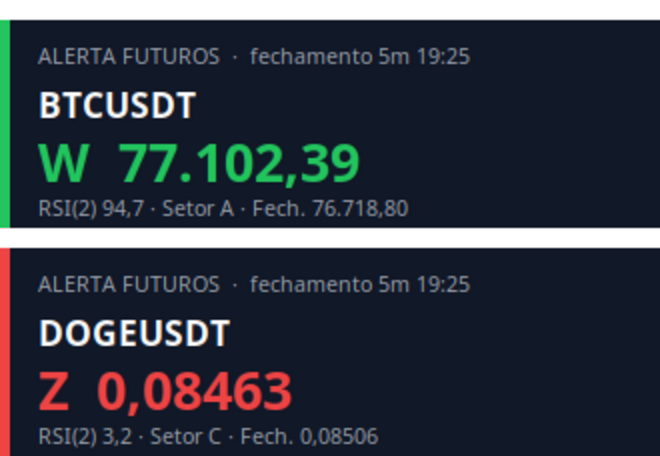
\includegraphics[width=\linewidth]{popups-poc.png}\\[1mm]
    {\scriptsize\color{txtgray} Captura real dos pop-ups da PoC (valores de demonstração).}
  \end{tcolorbox}
  \begin{tcolorbox}[enhanced, colback=white, colframe=borderc, arc=4pt, boxsep=4pt, add to width=-6mm,
                    title={Resultados medidos ao vivo}, colbacktitle=lightbg, coltitle=navy, fonttitle=\bfseries\small]
    \small
    \renewcommand{\arraystretch}{1.28}
    \begin{tabularx}{\linewidth}{@{}X r@{}}
      Período         & \pocMin\ min \\
      Pares simultâneos & 8 \\
      Fechamentos & \textbf{\pocAval} \\
      Sinais (X ou Y) & \textbf{\pocSinais} \\
      Latência mediana & \textbf{\pocLatMed\ ms} \\
      Latência (95\%) & \pocLatPnf\ ms \\
      Latência máxima & \pocLatMax\ ms \\
      Quedas recuperadas & \pocReconex\ de \pocReconex \\
      Memória / CPU & \pocRam\ MB / $<$1\% \\
      Testes automáticos & 14/14 \icoCheck \\
      Queda simulada & aprovado \icoCheck \\
    \end{tabularx}

    \vspace{1mm}
    {\scriptsize\color{txtgray} Execução em \pocData, rede residencial em Blumenau/SC.}
  \end{tcolorbox}
\end{tcbraster}

Trecho real do registro da PoC: o fechamento das 20:15, com 6 sinais em 8 pares (cada linha é um par avaliado):

\begin{tcolorbox}[terminal]
\begin{Verbatim}[breaklines=false]
20:15 SOLUSDT   fech       97,73 | RSI(2)  92,8 ACIMA  | 15m 0,442% setor A      | lat 316 ms  >>> SINAL X: alvo W 98,22
20:15 LTCUSDT   fech       51,07 | RSI(2)  92,9 ACIMA  | 15m 0,314% setor A      | lat 450 ms  >>> SINAL X: alvo W 51,33
20:15 XRPUSDT   fech      1,2872 | RSI(2)  71,5        | 15m 0,319% setor A      | lat 520 ms
20:15 LINKUSDT  fech      10,904 | RSI(2)  90,6 ACIMA  | 15m 0,423% setor A      | lat 520 ms  >>> SINAL X: alvo W 10,959
20:15 DOGEUSDT  fech     0,08011 | RSI(2)  89,3        | 15m 0,351% setor A      | lat 649 ms
20:15 BNBUSDT   fech      720,78 | RSI(2)  93,9 ACIMA  | 15m 0,280% setor A      | lat 649 ms  >>> SINAL X: alvo W 724,38
20:15 BTCUSDT   fech   75.817,70 | RSI(2)  93,6 ACIMA  | 15m 0,278% setor A      | lat 724 ms  >>> SINAL X: alvo W 76.196,79
20:15 ETHUSDT   fech    2.397,78 | RSI(2)  92,4 ACIMA  | 15m 0,383% setor A      | lat 823 ms  >>> SINAL X: alvo W 2.409,77
\end{Verbatim}
\end{tcolorbox}

\begin{tcolorbox}[cyanbox]
  \small\textbf{A PoC já achou e corrigiu um problema real:} numa queda de conexão às 19:50, o app
  reconectou sozinho em 4 s, mas a vela fechada durante a queda não era avaliada. Corrigido e comprovado
  com um teste que derruba a conexão na virada da vela. O RSI confere com a referência de Wilder (19/19).
\end{tcolorbox}

% ══════════════════════════════════════════════════════════════════════
\section{Ajustes Técnicos Importantes}
% ══════════════════════════════════════════════════════════════════════

Durante a PoC, identificamos pontos em que o documento precisa de um pequeno ajuste para
funcionar exatamente como você espera. \textbf{Nenhum muda a sua estratégia} --- eles garantem
que os números do app batam com o que você vê no gráfico da Binance.

\begin{tcolorbox}[ajuste, title={4.1 \enspace RSI de 2 períodos precisa de mais do que 2 velas}]
  \small O documento pede o histórico das \textbf{2 últimas velas}. Porém o RSI dos gráficos usa uma
  média suavizada que carrega o efeito das velas anteriores: calculado com só 2 ou 3 velas, o valor
  \textbf{fica diferente do gráfico}. \textbf{Solução:} ao abrir, o app baixa 300 velas de 5m por par
  (as últimas 25 horas) em uma única consulta, e o RSI já nasce idêntico ao do gráfico.
\end{tcolorbox}

\begin{tcolorbox}[ajuste, title={4.2 \enspace Endereços da Binance mudaram em abril de 2026}]
  \small Os endereços do documento (\texttt{https://binance.com} e \texttt{wss://://binance.com})
  não funcionam, e muitos tutoriais antigos também estão desatualizados: desde
  \textbf{23/04/2026} a Binance só envia velas de Futuros pela rota \texttt{/market}. Pela rota
  antiga, a conexão abre, mas \textbf{nenhuma vela chega} --- o app ficaria mudo, sem dar erro.
  A PoC já usa os endereços corretos: \texttt{fapi.binance.com/fapi/v1/klines} e
  \texttt{fstream.binance.com/market/stream}.
\end{tcolorbox}

\begin{tcolorbox}[ajuste, title={4.3 \enspace ``Latência zero'': o que é fisicamente possível}]
  \small Nenhum programa recebe a vela antes de a Binance publicá-la. Medimos cada parte do tempo
  entre o fechamento da vela e o alerta:
  \begin{itemize}[leftmargin=1.4em, itemsep=1pt, topsep=2pt]
    \item[\icoBullet] \textbf{Binance publicar a vela fechada:} de 0,1 a 3 s, conforme o par e o momento;
    \item[\icoBullet] \textbf{Internet até os servidores da Binance (Japão):} cerca de 250 ms;
    \item[\icoBullet] \textbf{Cálculo no app:} menos de 1 ms.
  \end{itemize}
  Na execução de 60 minutos, o alerta apareceu em \textbf{\pocLatMed\ ms na mediana} e em até
  \textbf{3,2 s em 95\% dos casos} --- os mais lentos quase sempre no LTCUSDT, o par menos negociado
  dos oito. Esse é o limite para qualquer linguagem ou tecnologia; por isso a escolha da linguagem não
  muda a velocidade (Seção 6).
\end{tcolorbox}

\begin{tcolorbox}[ajuste, title={4.4 \enspace Notificação nativa do Windows não aceita cores nem 10 s exatos}]
  \small A notificação padrão do Windows (\emph{toast}) usa sempre as cores do sistema, e o tempo de
  exibição é definido pelo próprio Windows. \textbf{Solução:} um pop-up próprio, com a mesma
  aparência e posição (canto inferior direito), preço em \textbf{\textcolor{sinalW}{verde}} ou
  \textbf{\textcolor{sinalZ}{vermelho}}, fechamento automático em 10 s e empilhamento quando
  vários pares disparam juntos. O alerta também fica registrado na Central de Notificações do
  Windows, como histórico.
\end{tcolorbox}

\begin{tcolorbox}[ajuste, title={4.5 \enspace Definições a confirmar com você}]
  \small
  \begin{enumerate}[leftmargin=1.4em, itemsep=2pt, topsep=1pt, label=\textbf{\alph*)}]
    \item \textbf{Tamanho mínimo de 0,020\%:} consideramos (Máxima $-$ Mínima) $\div$ Mínima.
    \item \textbf{Fechamentos de :00, :15, :30 e :45:} nesses horários a vela de 15m também fecha.
      Usamos a vela de 15m que \textbf{termina junto} com a de 5m (a que contém o preço avaliado).
    \item \textbf{Limites:} RSI exatamente 90 conta como Acima; exatamente 5, como Abaixo. O
      preço exatamente na divisa de um setor conta como dentro do setor A ou C.
    \item \textbf{Menu ``Setor da vela de 15m'' (Superior, Médio, Inferior):} a regra de cruzamento
      fixa X = Setor A e Y = Setor C. Sugerimos manter a regra fixa e permitir ajustar o
      \textbf{tamanho} dos setores (30\%) na janela. Se você quiser escolher outro setor, basta nos avisar.
  \end{enumerate}
\end{tcolorbox}

% ══════════════════════════════════════════════════════════════════════
\section{Escopo --- Versão 1}
% ══════════════════════════════════════════════════════════════════════

Seguindo o seu pedido de uma primeira versão \textbf{simples, sem extras}, oferecemos duas
opções. As duas têm o mesmo motor de alertas; a diferença é a janela de configuração.

\begin{tcbraster}[raster columns=2, raster equal height, raster column skip=5mm]
  \begin{tcolorbox}[opcao, title={Opção A --- Essencial}]
    \centering{\color{navymid}\Large\bfseries R\$ \valA}\\[1mm]
    {\scriptsize\color{txtgray} o essencial, sem janela de configuração}\par\vspace{2mm}\raggedright
    \small
    \begin{itemize}[leftmargin=1.3em, itemsep=2pt, topsep=0pt]
      \item[\icoCheck] Monitoramento dos 8 pares, 24 h
      \item[\icoCheck] Toda a regra do documento (Seção 2)
      \item[\icoCheck] Pop-up verde/vermelho por 10 s
      \item[\icoCheck] Reconexão automática
      \item[\icoCheck] Roda em segundo plano, com ícone perto do relógio: \emph{Iniciar}, \emph{Parar} e \emph{Sair}
      \item[\icoCheck] Registro CSV de fechamentos e sinais
      \item[\icoCheck] Executável \texttt{.exe} + instalação remota assistida
      \item[\icoCross] Parâmetros fixos (90/5, 30\%, 0,020\%, 0,5\%); alteração feita por nós, sob demanda
    \end{itemize}
  \end{tcolorbox}
  \begin{tcolorbox}[opcaorec, title={Opção B --- Completa}]
    \centering{\color{golddk}\Large\bfseries R\$ \valB}\\[1mm]
    {\scriptsize\bfseries\color{golddk}\ding{72} RECOMENDADA \ding{72}}\enspace{\scriptsize\color{txtgray}atende 100\% do documento}\par\vspace{2mm}\raggedright
    \small
    \textbf{Tudo da Opção A, mais a janela do documento:}
    \begin{itemize}[leftmargin=1.3em, itemsep=2pt, topsep=2pt]
      \item[\icoCheck] Campos para os limites do RSI (Acima / Abaixo)
      \item[\icoCheck] Campo para o tamanho dos setores A e C
      \item[\icoCheck] Campos para o tamanho mínimo da vela 15m e o fator de ajuste
      \item[\icoCheck] Botões \emph{Iniciar Monitoramento} e \emph{Parar Monitoramento}
      \item[\icoCheck] Quadro de situação: último RSI, setor e horário de cada par, e status da conexão
      \item[\icoCheck] Configurações salvas entre usos
      \item[\icoCheck] Opção de iniciar junto com o Windows
    \end{itemize}
  \end{tcolorbox}
\end{tcbraster}

\begin{tcolorbox}[goldbox]
  \small\textbf{Por que recomendamos a Opção B:} o documento pede a janela com campos e botões, e ela
  permite testar variações da estratégia (por exemplo, RSI 95/3 ou setores de 25\%) \textbf{sem
  depender de nós} e sem custo de alteração.
\end{tcolorbox}

% ══════════════════════════════════════════════════════════════════════
\section{Tecnologia}
% ══════════════════════════════════════════════════════════════════════

\begin{center}
\small
\renewcommand{\arraystretch}{1.3}
\begin{tabularx}{\textwidth}{@{}>{\bfseries}p{40mm} X@{}}
  \toprule
  \rowcolor{navy!8}
  \textbf{Componente} & \textbf{Escolha} \\
  \midrule
  Linguagem          & Python 3 --- a mesma da PoC, que evolui para o produto final (menor custo) \\
  Conexão Binance    & REST \texttt{fapi.binance.com} + WebSocket \texttt{fstream.binance.com/market} \\
  Cálculos           & Implementação própria do RSI de Wilder e dos setores, com testes automáticos \\
  Janela e pop-ups   & Tkinter (nativo do Python): leve e sem dependências extras \\
  Distribuição       & Executável único \texttt{.exe} (PyInstaller) --- não exige instalar Python \\
  Requisitos do laptop & Windows 10 ou 11, internet estável, cerca de 50 MB de memória livre \\
  \bottomrule
\end{tabularx}
\end{center}

\textbf{E C\# / .NET ou Node.js?} Também atenderiam, mas, como mostrado no ajuste 4.3, o tempo do
alerta depende da Binance e da internet, não da linguagem. Python permite aproveitar a PoC já
testada e entregar mais rápido e com custo menor. Se você preferir C\#, podemos orçar à parte.

% ══════════════════════════════════════════════════════════════════════
\section{Cronograma}
% ══════════════════════════════════════════════════════════════════════

\begin{center}
\small
\renewcommand{\arraystretch}{1.35}
\begin{tabularx}{\textwidth}{@{}>{\bfseries\leavevmode\color{navymid}}p{30mm} X >{\raggedleft\arraybackslash}p{32mm}@{}}
  \toprule
  \rowcolor{navy!8}
  \textbf{\color{black}Etapa} & \textbf{Entregas} & \textbf{Prazo} \\
  \midrule
  1 --- PoC no laptop & Executável de teste instalado remotamente; roda por até 3 dias gravando todos os
    fechamentos em planilha; reunião de 30 min para conferir os valores com o gráfico da Binance e
    fechar as definições do item 4.5 & 2 dias úteis \\
  2 --- Versão 1 & Opção escolhida (A ou B) desenvolvida, testada em Windows 10 e 11 e empacotada em \texttt{.exe} & A: 4 / B: 7 dias úteis \\
  3 --- Entrega & Instalação remota assistida, guia rápido de uso em PDF e 30 min de orientação & 1 dia útil \\
  \midrule
  \rowcolor{gold!12}
  \textbf{\color{black}Total} & Da aprovação da PoC até o app instalado & \textbf{A: 5 / B: 8 dias úteis} \\
  \bottomrule
\end{tabularx}
\end{center}

% ══════════════════════════════════════════════════════════════════════
\section{Investimento}
% ══════════════════════════════════════════════════════════════════════

\begin{center}
\renewcommand{\arraystretch}{1.45}
\begin{tabularx}{\textwidth}{@{}X r r@{}}
  \toprule
  \rowcolor{navy!8}
  \textbf{Item} & \textbf{Opção A} & \textbf{Opção B} \\
  \midrule
  \textbf{Etapa 1 --- PoC instalada no seu laptop}      & R\$ \valPoc & R\$ \valPoc \\
  \textbf{Etapas 2 e 3 --- Versão 1 + entrega}          & R\$ \valAsaldo & R\$ \valBsaldo \\
  \quad Motor de alertas, pop-ups, reconexão, registro CSV & incl. & incl. \\
  \quad Ícone em segundo plano (Iniciar / Parar / Sair)   & incl. & incl. \\
  \quad Janela de configuração e quadro de situação       & ---   & incl. \\
  \quad Executável, instalação remota e guia de uso       & incl. & incl. \\
  \quad Garantia de 60 dias para correção de erros        & incl. & incl. \\
  \midrule
  \rowcolor{navy!14}
  \textbf{\large Total do projeto} & \textbf{\large R\$ \valA} & \textbf{\large R\$ \valB} \\
  \bottomrule
\end{tabularx}
\end{center}

\begin{tcolorbox}[greenbox]
  \small\textbf{Sem risco na primeira etapa:} se, após testar a PoC no seu laptop, você decidir não
  seguir, paga apenas os R\$ \valPoc. Se seguir, esse valor já está \textbf{descontado} do total.
\end{tcolorbox}

\begin{tcolorbox}[pricebox, title={\color{navy}\icoStar\enspace Suporte e Evolução (opcional, após a garantia)}, colbacktitle=gold]
  \renewcommand{\arraystretch}{1.35}
  \begin{tabularx}{\linewidth}{@{}X r@{}}
    \textbf{Plano mensal:} adaptação a mudanças da Binance (como a de abril/2026), pequenos ajustes de
    parâmetros e suporte por WhatsApp & \textbf{\color{gold}R\$ \valSuporte/mês} \\
    \textbf{Novas funções} (outros pares, som, Telegram etc.) & R\$ \valHora/hora \\
  \end{tabularx}
\end{tcolorbox}

\subsection{Condições de Pagamento}

\begin{itemize}[leftmargin=1.8em, itemsep=3pt]
  \item[\icoCheck] \textbf{Etapa 1 (PoC):} R\$ \valPoc\ no aceite desta proposta.
  \item[\icoCheck] \textbf{Etapas 2 e 3:} 50\% no início da Versão 1 e 50\% na entrega:
    Opção~A em 2~\texttimes~R\$~\valAparc; Opção~B em 2~\texttimes~R\$~\valBparc.
\end{itemize}
Pagamentos via \textbf{PIX} (CNPJ \textbf{53.700.754/0001-10}), com emissão de nota fiscal.

% ══════════════════════════════════════════════════════════════════════
\section{Premissas, Fora de Escopo e Aviso de Risco}
% ══════════════════════════════════════════════════════════════════════

\begin{tcbraster}[raster columns=2, raster equal height, raster column skip=5mm]
  \begin{tcolorbox}[enhanced, colback=white, colframe=borderc, arc=4pt, title={Premissas}, colbacktitle=lightbg, coltitle=navy, fonttitle=\bfseries\small]
    \small
    \begin{itemize}[leftmargin=1.2em, itemsep=2pt, topsep=0pt]
      \item[\icoBullet] Laptop ligado, fora do modo de suspensão e com internet enquanto monitora.
      \item[\icoBullet] A rede do cliente acessa os servidores públicos da Binance.
      \item[\icoBullet] Acesso remoto (AnyDesk ou similar) para instalação.
      \item[\icoBullet] Retorno sobre a PoC em até 5 dias úteis.
      \item[\icoBullet] Regra de sinais conforme o documento e o item 4.5.
    \end{itemize}
  \end{tcolorbox}
  \begin{tcolorbox}[enhanced, colback=white, colframe=borderc, arc=4pt, title={Fora de escopo}, colbacktitle=lightbg, coltitle=navy, fonttitle=\bfseries\small]
    \small
    \begin{itemize}[leftmargin=1.2em, itemsep=2pt, topsep=0pt]
      \item[\icoCross] Envio de ordens, conta ou API key.
      \item[\icoCross] Outros pares, tempos gráficos ou indicadores.
      \item[\icoCross] Teste histórico da estratégia (backtest).
      \item[\icoCross] Celular, macOS, Telegram, e-mail ou som.
      \item[\icoCross] Certificado de assinatura digital: sem ele, o Windows mostra um aviso
        na primeira execução, que basta confirmar.
    \end{itemize}
  \end{tcolorbox}
\end{tcbraster}

\begin{tcolorbox}[goldbox]
  \small\textbf{Aviso de risco.} O Alerta Futuros é uma ferramenta \textbf{informativa}: aplica
  automaticamente a regra definida pelo cliente e não constitui recomendação de investimento.
  A estratégia, os parâmetros e qualquer decisão de operar são de responsabilidade exclusiva do
  cliente. Contratos futuros envolvem alto risco. O app depende da disponibilidade dos serviços
  públicos da Binance, que podem mudar ou ficar indisponíveis sem aviso prévio.
\end{tcolorbox}

% ══════════════════════════════════════════════════════════════════════
\section{Termos e Aceite}
% ══════════════════════════════════════════════════════════════════════

\begin{itemize}[leftmargin=1.8em, itemsep=2pt]
  \item Proposta válida por \textbf{30 dias} a partir de 16 de setembro de 2026.
  \item Valores em Reais (BRL), com nota fiscal.
  \item \textbf{Garantia de 60 dias} após a entrega para correção de erros, sem custo.
  \item O executável e o código-fonte são entregues ao cliente após a quitação.
  \item Mudanças de escopo são combinadas por escrito, com prazo e valor definidos antes.
\end{itemize}

\vspace{2mm}
\textbf{Opção escolhida:} \quad $\square$ Opção A --- Essencial (R\$ \valA) \qquad $\square$ Opção B --- Completa (R\$ \valB)

\vspace{9mm}
\noindent
\begin{minipage}[t]{0.47\textwidth}
  \centering
  \rule{\linewidth}{0.4pt}\\[2mm]
  \textbf{\autor}\\[1mm]
  {\small Blumenau\,\textcolor{golddk}{\textbf{TI}} \textbullet\ CNPJ 53.700.754/0001-10}\\[1mm]
  {\scriptsize\href{\autorLinkedinURL}{\color{navymid}\autorLinkedin}}\\[2mm]
  {\small Blumenau, 16 de setembro de 2026}
\end{minipage}
\hfill
\begin{minipage}[t]{0.47\textwidth}
  \centering
  \rule{\linewidth}{0.4pt}\\[2mm]
  \textbf{\cliente}\\[1mm]
  {\small Contratante}\\[2mm]
  {\small CPF: \rule{3.2cm}{0.3pt}\quad Data: \rule{0.6cm}{0.3pt}/\rule{0.6cm}{0.3pt}/2026}
\end{minipage}

\vspace{5mm}
\begin{tcolorbox}[greenbox]
  \small\textbf{Para aceitar ou tirar dúvidas:} WhatsApp \textbf{+55 47 98867-7798} \;\textbullet\;
  contato@blumenauti.com.br \;\textbullet\; \href{https://www.blumenauti.com.br}{www.blumenauti.com.br}.
  Aceite também por resposta escrita (e-mail ou WhatsApp) indicando a opção escolhida.
\end{tcolorbox}

\end{document}
